%************************************************
\chapter{Watch It Grow}
%************************************************

\section{Sentimental Introduction\protect\footnote{This section can be skipped, without any loss of continuity.}}
	Science often seems like a blackbox that relates observables. Even more often, it is rather convenient to lose touch of observables altogether, and wander in the blackbox. Performing an experiment, gets one closer to nature, to the roots of the subject.

\section{The Journey}
	\subsection{Look it has begun}
		This experiment wasn't started from scratch. My guide, \myProf, had already worked with a team and created the Dipoles as described earlier. The team had also worked on the image detection algorithms, but their work wasn't usable.
		\par
		There were three tasks at hand, of which one had been significantly simplified by the prior work.
		\begin{enumerate}
			\item The Dipole
					\par
					This had one apparent problem; the dipoles had to be made virtually frictionless (which is not to say they had excessive friction, infact they would oscillate atleast about 8 times before stopping aligned with earth's magnetic field)
			\item The Image Analysis
					\par
					This part I had to start from the beginning with two basic objectives, as stated earlier; measuring the angle of the dipoles and evaluating the current to be pumped based on the temperature selected.\\
					What was known soon, was that C++ will be used for programming and linux would be the operating system, to facilitate USB interface with the AVR (next step)
			\item The Current Control Hardware
					\par
					This is simply for providing a current pulse proportional to the intensity calculated by the lattice analyser. Some schematics for this were available, but were found to be inaccurate and incomplete.
		\end{enumerate}
	
	\subsection{Time Line}
		\autoref{timeLine} is the event log, which has the progress as and when it was made.		
	
	\subsection{Construction of the Dipole}
		To remove the friction, there were various ideas, including use of a super conductor. However, eventually three methods were considered and experimentally tested.
		\begin{enumerate}
			\item Ferro-Fluid: 
					\par
					As it turns out, there are substances that have a ferro magnetic properties but in the liquid form. Consequently, a strong enough magnet would glide if coated with this substance.
					\par
					Experimentally, it was found that the friction was higher than the `needle on glass' setup. 
			\item Magnetic Levitation:
					\par
					A magnet can easily suspend another magnet, granted it doesn't flip. This idea was used and a magnetic cylinder was placed co-axial to the needle, using a cylindrical eraser and glue. Beneath the glass slide, an identical magnet was placed with the face that repels upwards.
					\par
					Experimentally, again it was found that the motion was more damped than the `needle on glass' setup. The reason for this case was obvious after a little analysis and closer observation. The dipole would align to the field of the magnet, viz. the magnetic field was interfering with the dipole.
			\item Air Levitation:
					\par
					To test this, the very first requirement was a source of stream of air. For this, we started small. We arranged for a small USB fan from a colleague. The next task was to channel the flow of air. This was accomplished by attaching the front part of a Pepsi Bottle such that the larger diameter was closer to the fan and the mouth of the bottle had the chord stuck to it (could still be moved if required), as diagrammatically given in \autoref{fanSetup}. The final setup has been given in \autoref{fanSetupActual}.
					\begin{figure}[bth]
						\begin{center}
							
\includegraphics[width=0.7\linewidth]{gfx/fanSetup.jpg}
						\end{center}
					\caption[Fan Setup]{Fan Setup}
					\label{fanSetup}
					\end{figure}

					\begin{figure}[bth]
						\begin{center}
							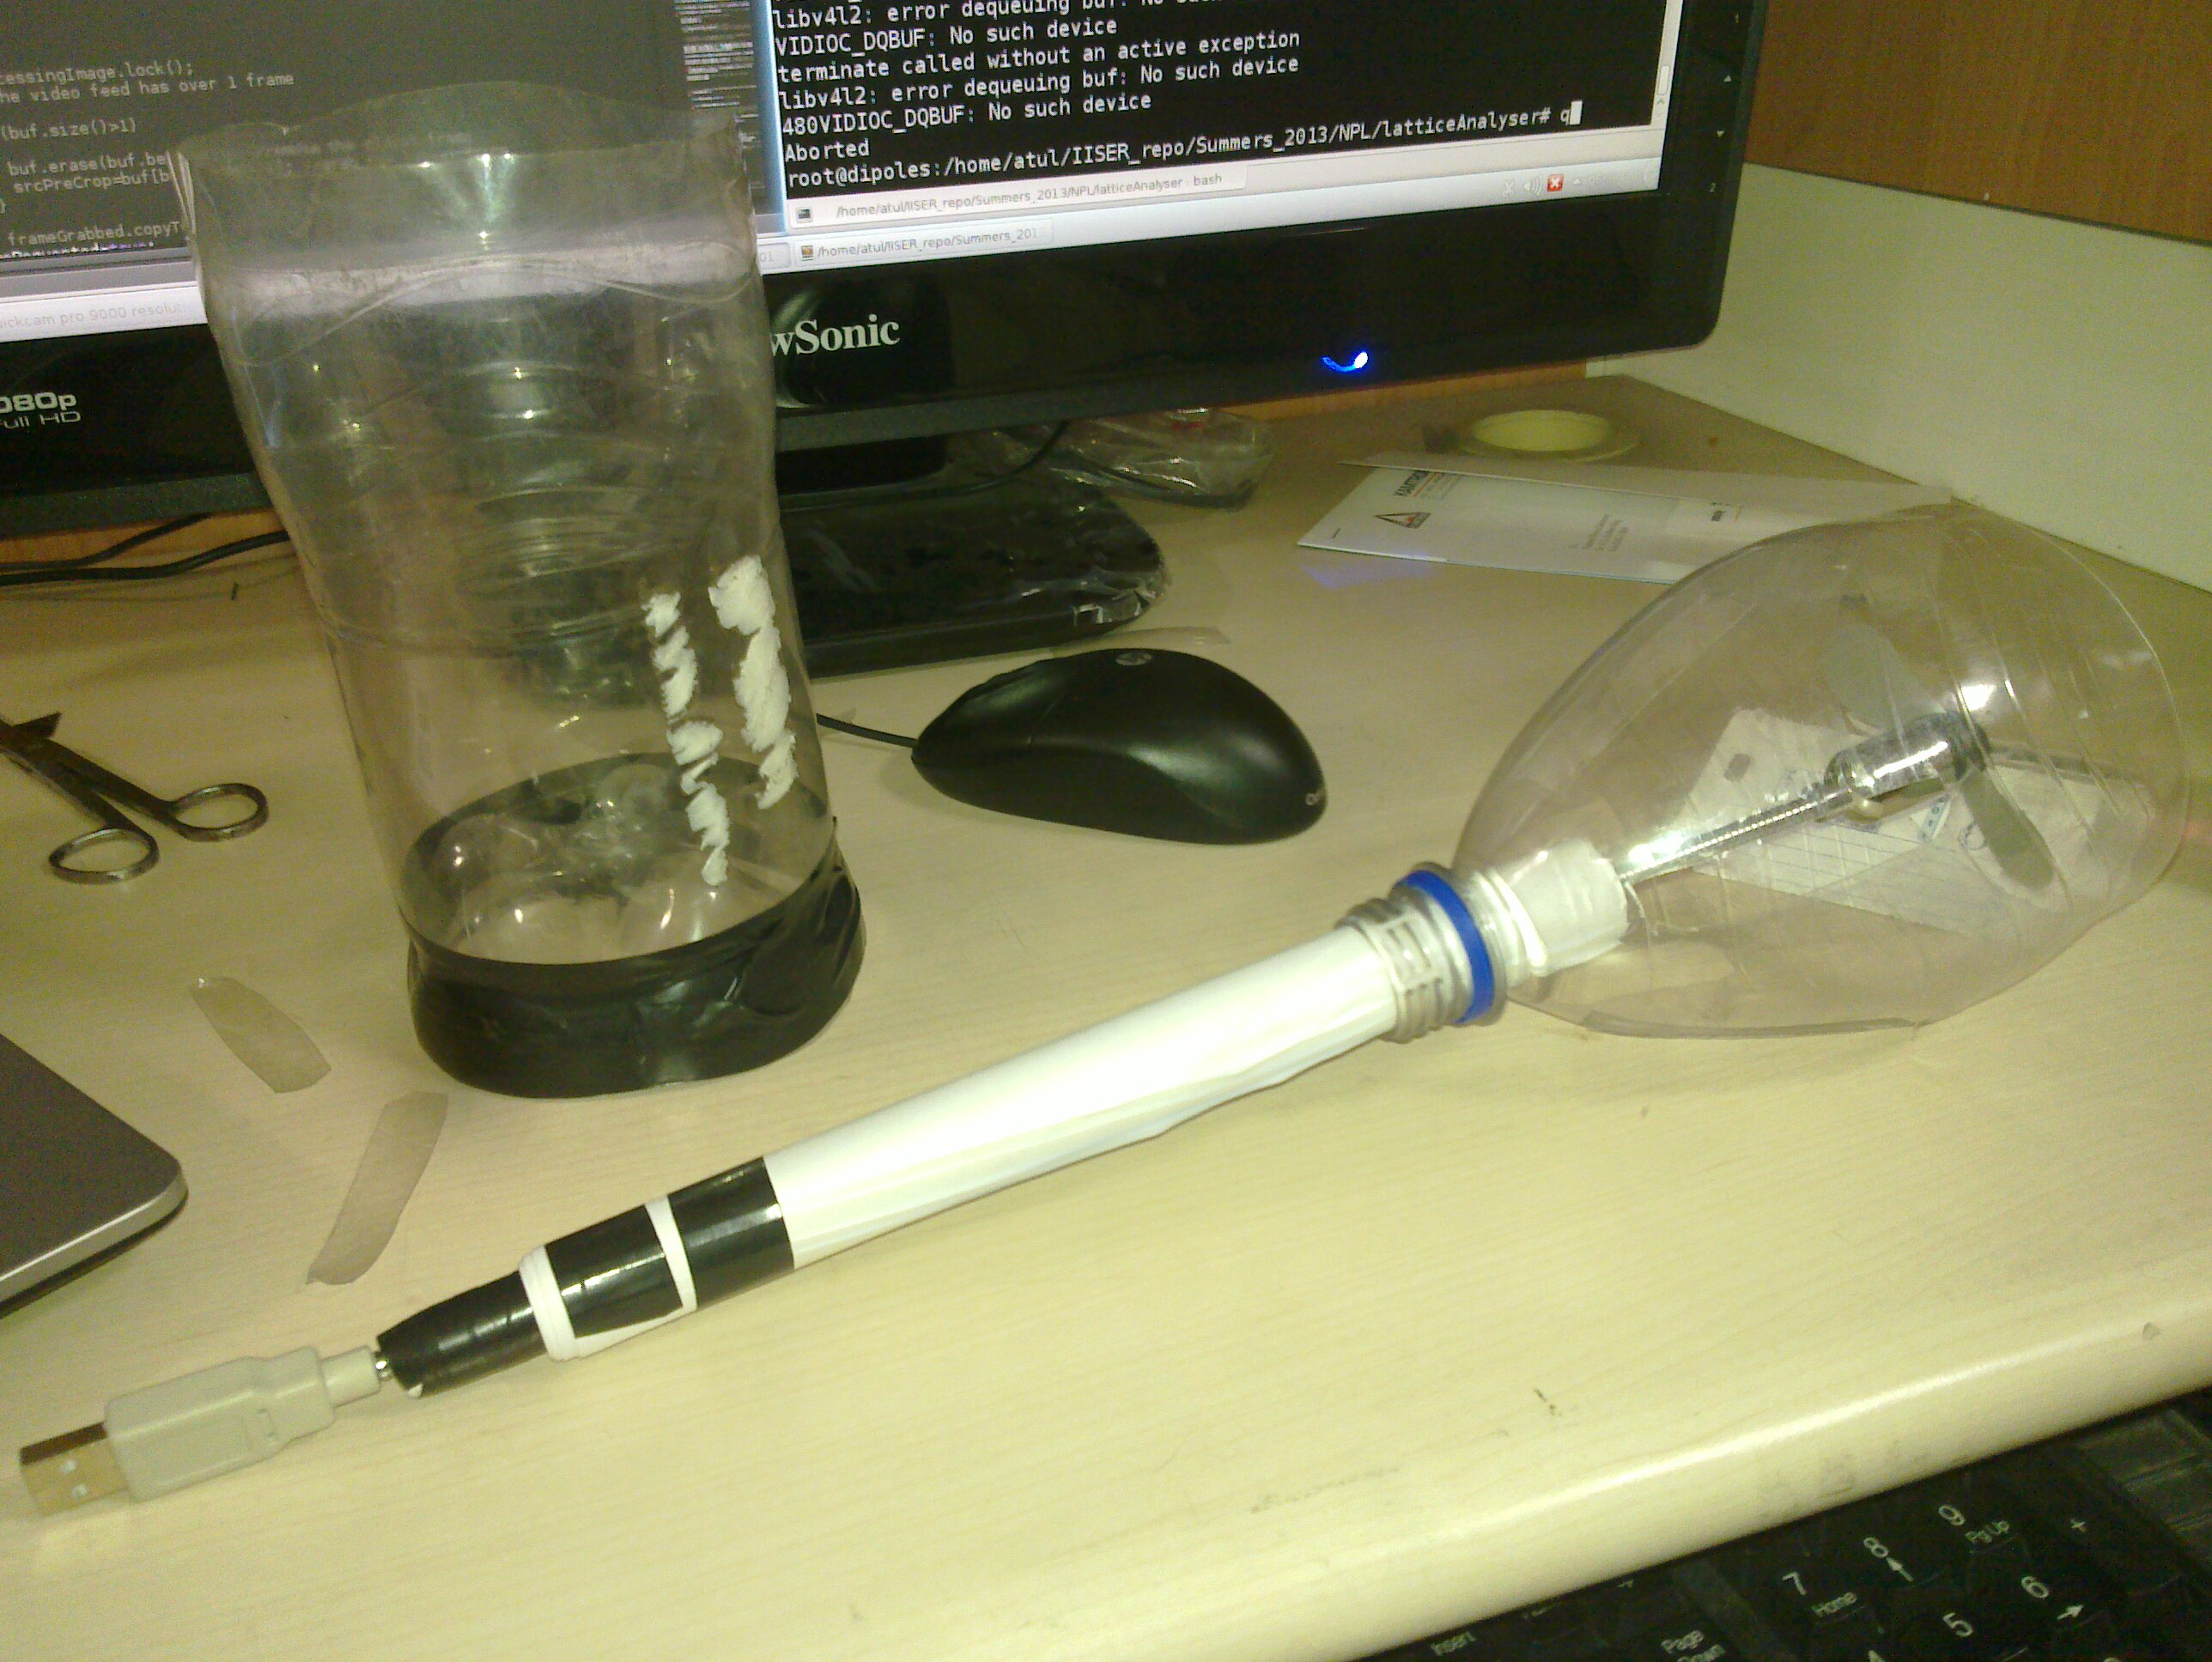
\includegraphics[width=0.7\linewidth]{gfx/fanSetupActual.jpg}
						\end{center}
					\caption[Final Fan Setup]{Final Fan Setup}
					\label{fanSetupActual}
					\end{figure}
					This failed miserably for the air pressure would fall the moment the assembly covered the fan. Introducing slits to allow air to flow in created no appreciable difference. This idea had to be dropped in favour of the vacuum cleaner setup as shown in \autoref{vacuumCleanerSetup}
					\begin{figure}[bth]
						\begin{center}
							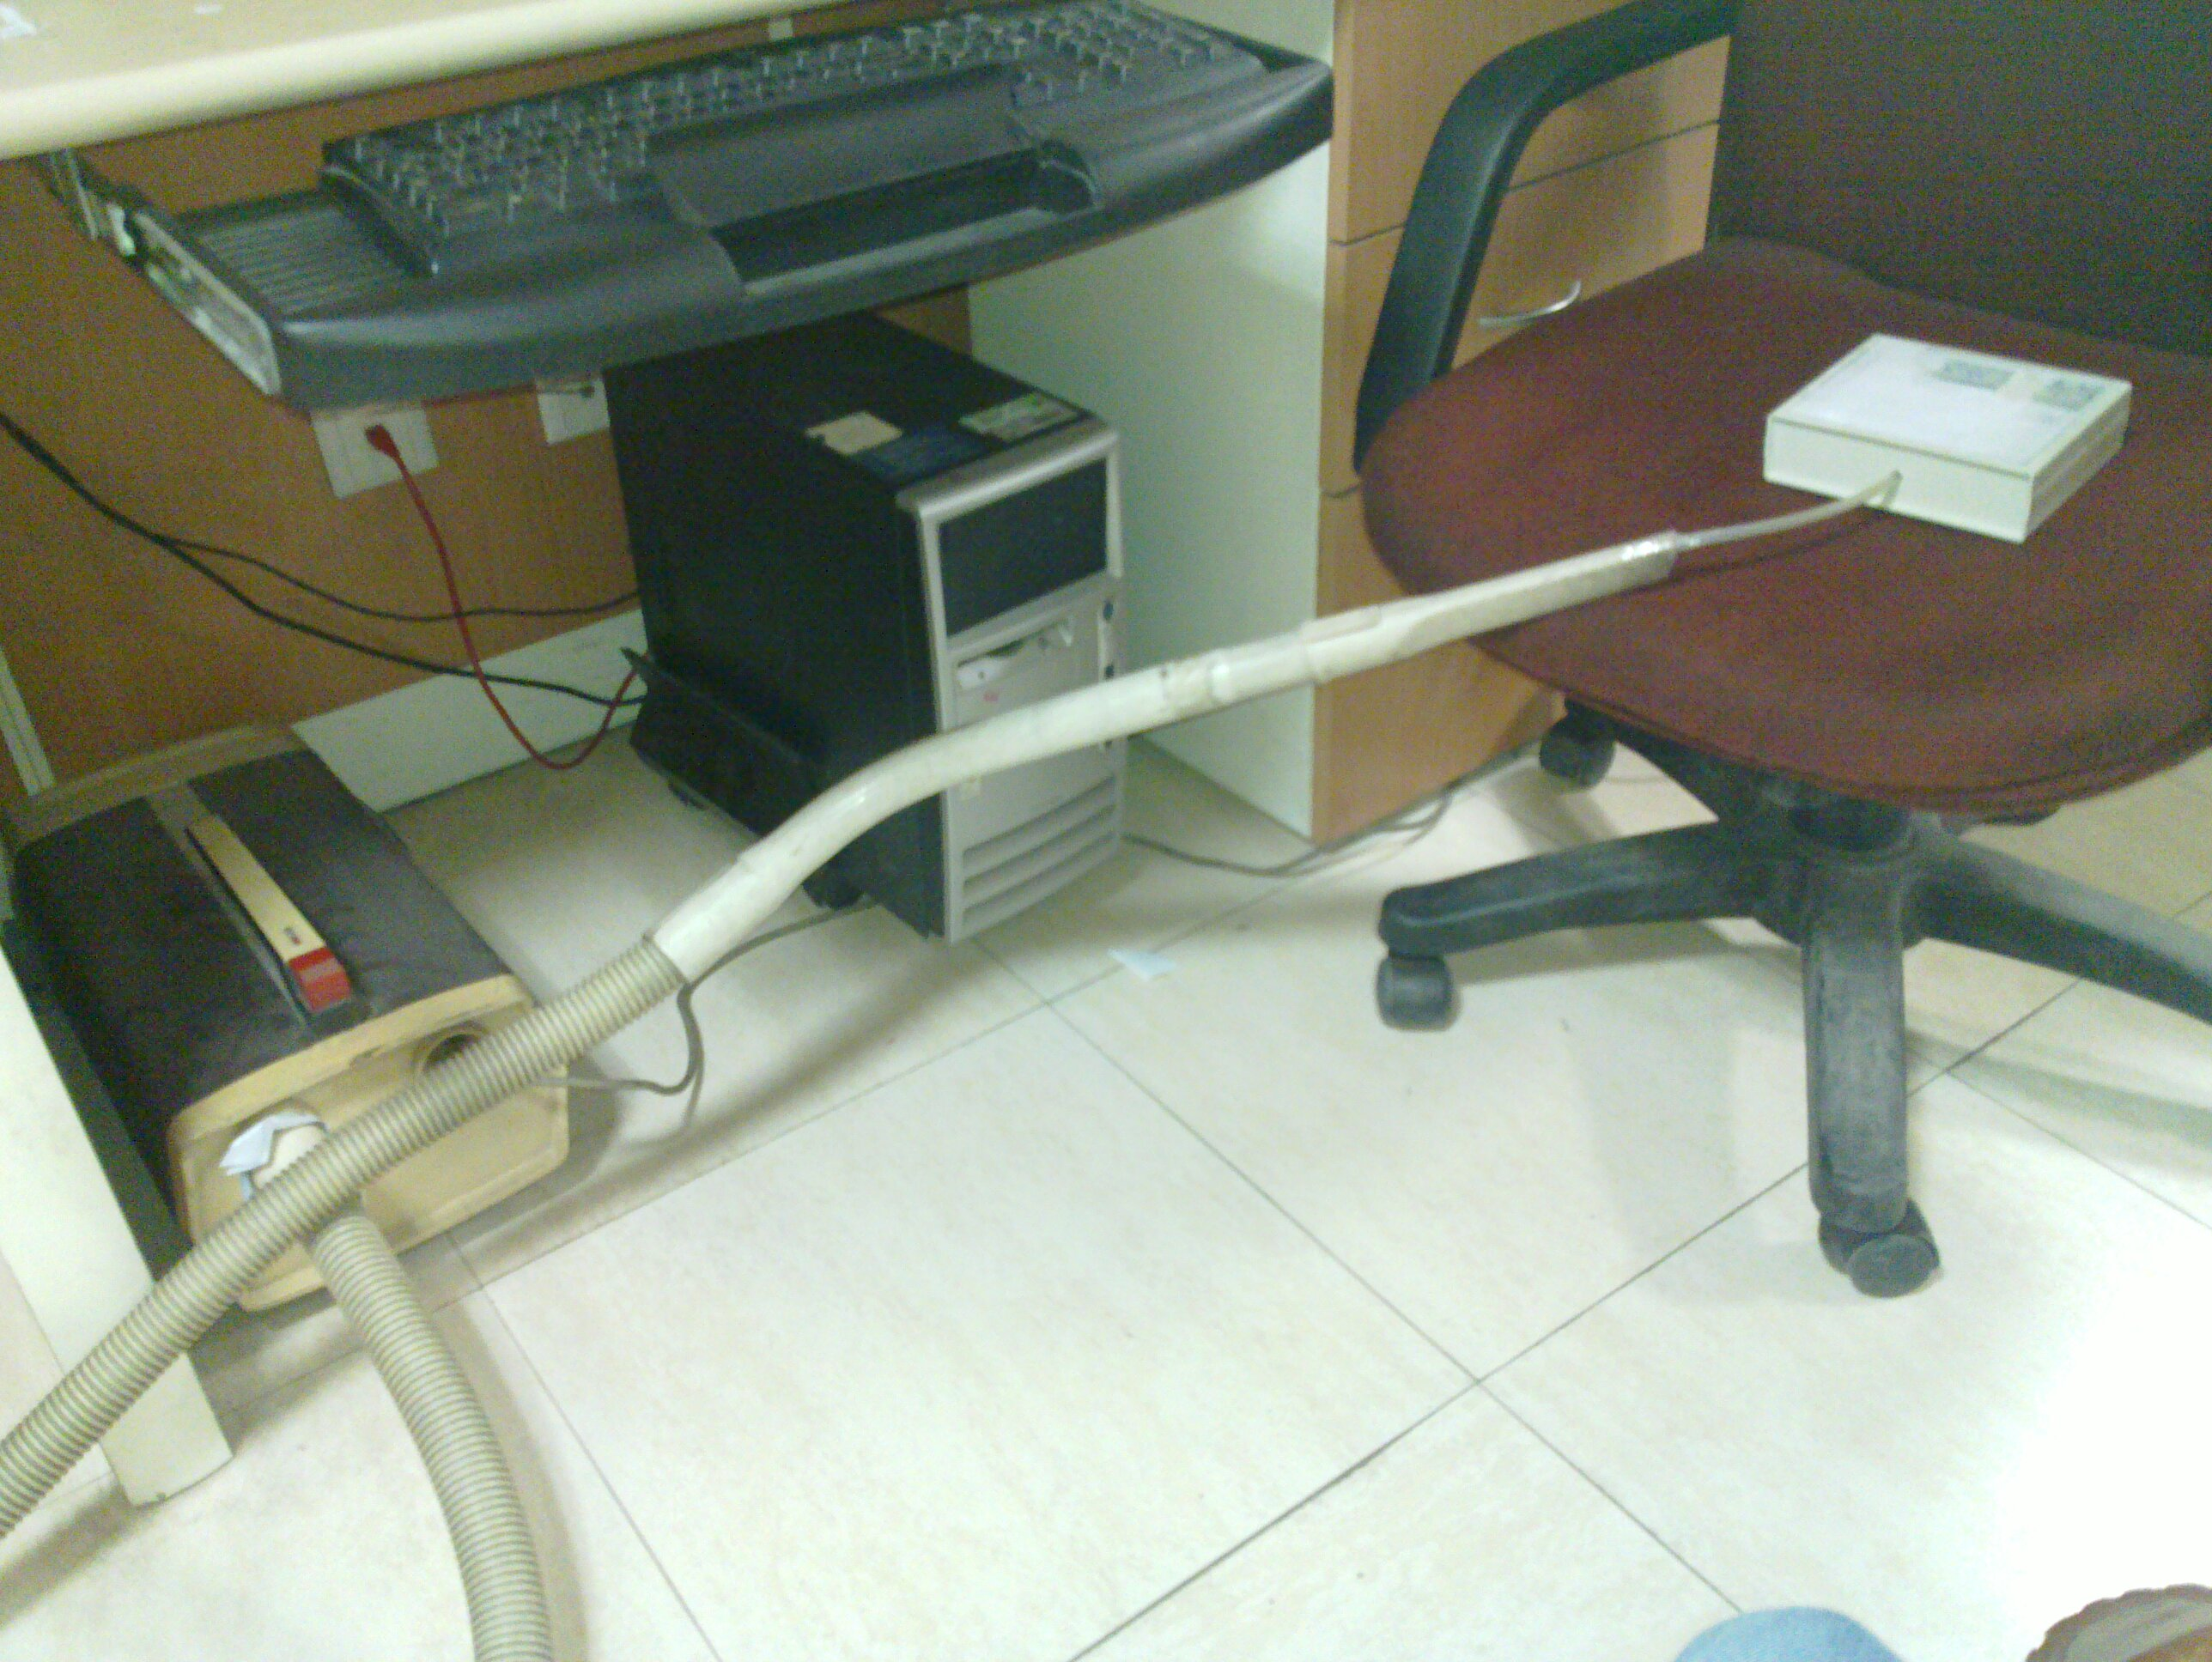
\includegraphics[width=0.7\linewidth]{gfx/vacuumCleanerSetup.jpg}
						\end{center}
					\caption[Vacuum Cleaner Setup]{Vacuum Cleaner Setup}
					\label{vacuumCleanerSetup}
					\end{figure}					 
					\par
					The vacuum cleaner was used as a blower and connected to a box using a pipe. On one of the faces of the box, four holes were drilled (which were later enlarged). These were covered to increase the pressure when required. On the open hole, one dipole was placed (which had to be re built with a minor modification, refer to \autoref{theLightDipole}) with a disc at the bottom. This is when an apparently bizarre observation was made. At a given pressure, it was found that the dipole could remain suspended in air beyond a certain height (and obviously there was an upper bound for the same). However, for heights lower than that, the dipole would fall. The explanation which seemed to resolve this was that the air could spread while rising sufficiently only beyond that height to apply pressure at a large enough surface area, thus create enough force. Albeit the experiment was not performed under precisely the same conditions, when it was repeated with a larger disc, the same problem was encountered, suggesting that there may be more to the explanation that deduced so far. Other geometries at the base (other than the disc) were also tried, such as a cone and a thermecol sphere, neither of which worked at low pressures which were enough to suspend the disc based setups. Further, at high pressures, disturbances in the form of torque in the dipole's axis of rotation begin to appear, which are fatal for the experiment.
					\begin{figure}[bth]
						\begin{center}
							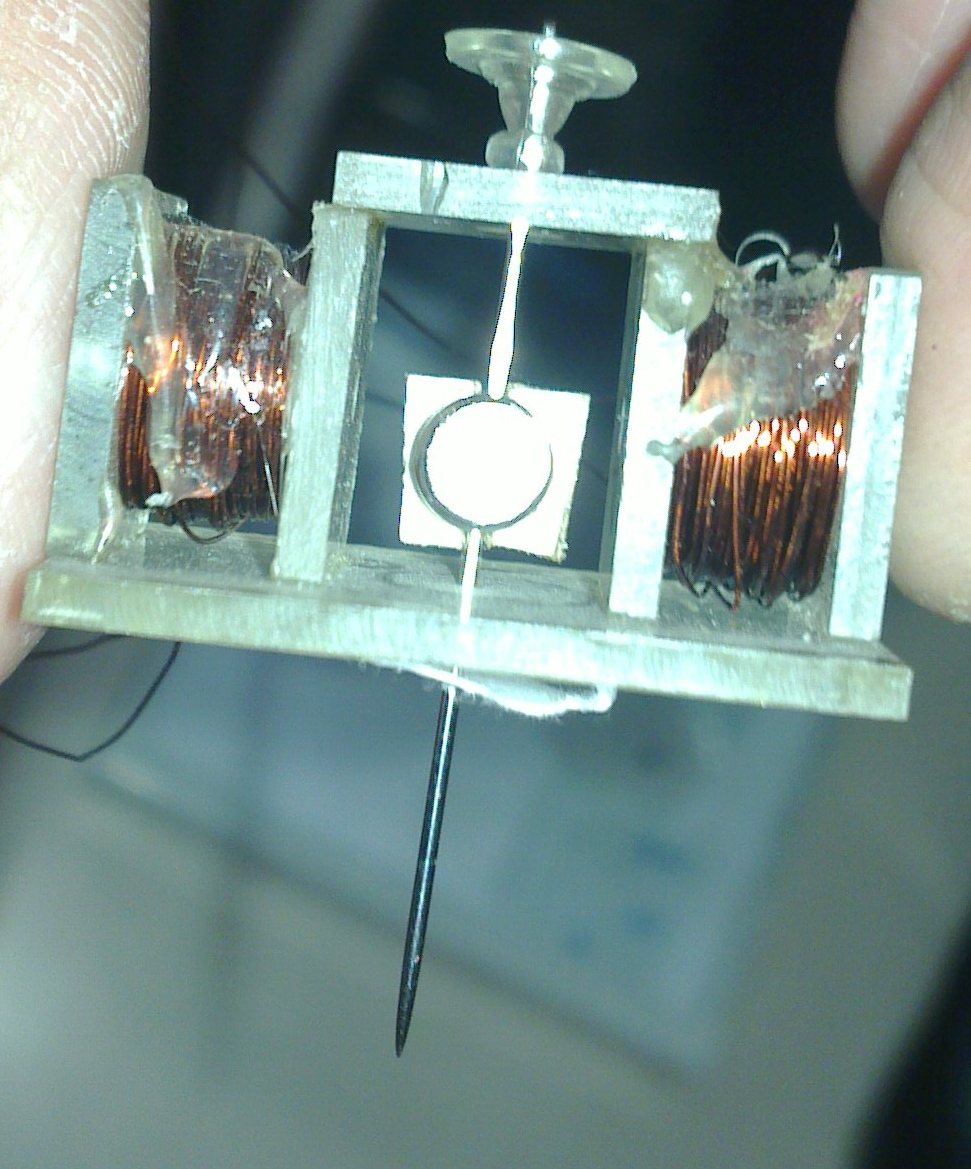
\includegraphics[width=0.7\linewidth]{gfx/theLightDipole.jpg}
						\end{center}
					\caption[The Modified Dipole]{The Modified Dipole}
					\label{theLightDipole}
					\end{figure}						
					\par
					Other problems with air-suspension included damping in the vertical direction. Once the dipole reaches the vertical equilibrium point, it overshoots just as an oscillator. Since the friction at the plates holding the needle vertical is negligible, the oscillations don't get damped quick enough. This was experimentally observed also. The energy ratio between the rotational part and the translation part, in the earth's field, was calculated and found to be approximately one for the given setup.
					\par
					The most stable we could achieve with this setup was using a cylindrical projection from which the high pressure air escapes and a disc of comparable size attached to the dipole. This did get suspended satisfactorily, unlike the other methods where the suspension could not be maintained at the desired height, however the needle became rather wobbly and unstable resulting in increased friction.
					\par
					Online research indicated that air-bearings do function well enough and so do the boards of air hockey. These will be explored in the coming weeks to improve upon the methods to achieve the desired results.
					\par
					THE DIPOLES
					\par
					Air hockey table method, DIY air hockey was a better method of searching, got cues
					\\
					aluminium disk's introduction (For air suspension), after finalizing one, and testing it, we found comparable resistance with the inverted needle top on glass slide as opposed to when air suspended. Hypothesised that the main source of friction was infact the guiding edges, which provide the opposing torque.
					\\
					an interesting setup was devised, with only the needle edges held using a glass slide and magnets. resist friction etc. 
					\\
					froze the design with aluminium disks at the bottom and made four good dipoles for testing in a 2x2 lattice
		\end{enumerate}
	\subsection{Construction of the Lattice Analyser}
		\subsubsection{Proof of Concept: Recognizing Patterns}
			The lattice analyser has come a long way. Image detection trials were initiated with \autoref{sampleImage}. 
			\begin{figure}[bth]
				\begin{center}
					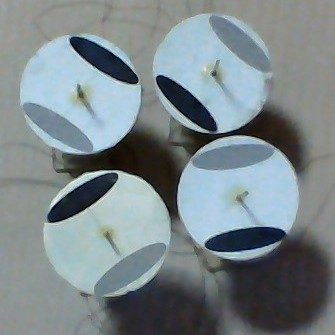
\includegraphics[width=0.7\linewidth]{gfx/picture002.jpg}
				\end{center}
			\caption[Sample Image]{Sample Image}
			\label{sampleImage}
			\end{figure}

			The idea was that once the ellipses have been detected, and they are different in colour, one can evaluate from their centroids, the position and the angle of the dipole. It must be stated that earlier it was attempted to use the greyscale image as was provided. However soon the shadow interference led to using coloured patterns instead. These patterns were not printed but displayed on a screen and the camera aimed appropriately.
			\par
			So first, the algorithm for detection of relevant part of the image had to be frozen. There were two candidates for this
			\begin{enumerate}
				\item Hough Transform Method
					\par
					Either one could use the already available in OpenCV, line detection or circle detection, both would've required changing the pattern on the dipole
					\par
					Or one could use an ellipse modification for the same, which would require programming the algorithm.
				\item Contour Detection and Ellipse Fitting
					\par
					This method detects contours in a given image, and the OpenCV example also shows ellipse fitting for the same. This seemed promising too, but it seemed more expensive (computationally) than looking for predetermined shapes.
			\end{enumerate}
			This work had been done within the first few days. 
			\par

			\begin{figure}[bth]
				\begin{center}
					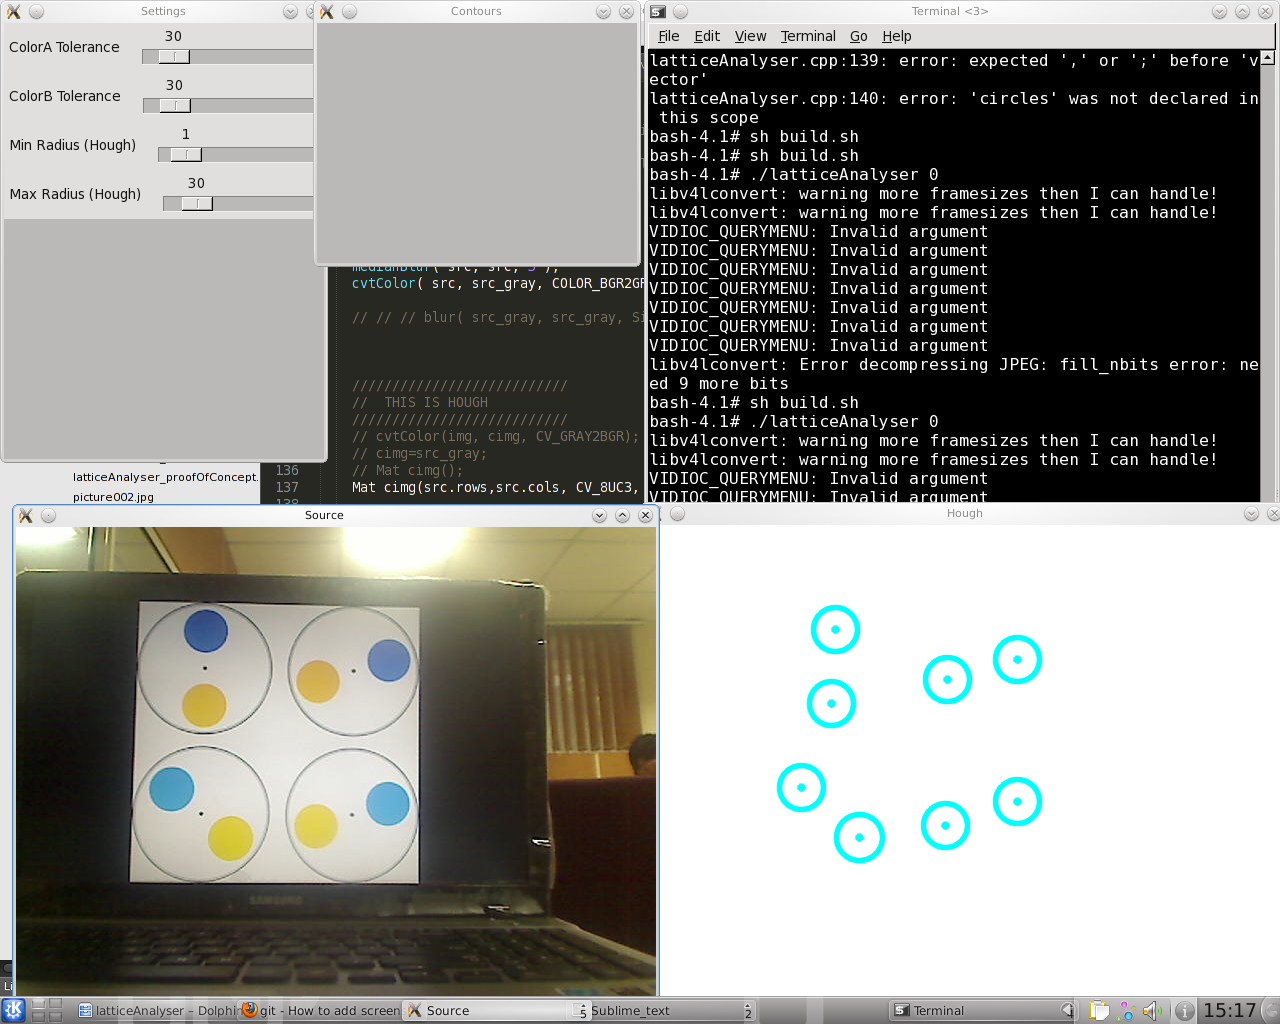
\includegraphics[width=1.1\linewidth]{../../latticeAnalyser/screenshots/snapshot1.png}
				\end{center}
			\caption[Hough Transform]{Hough Transform}
			\label{snapshot1}
			\end{figure}

			\begin{figure}[bth]
				\begin{center}
					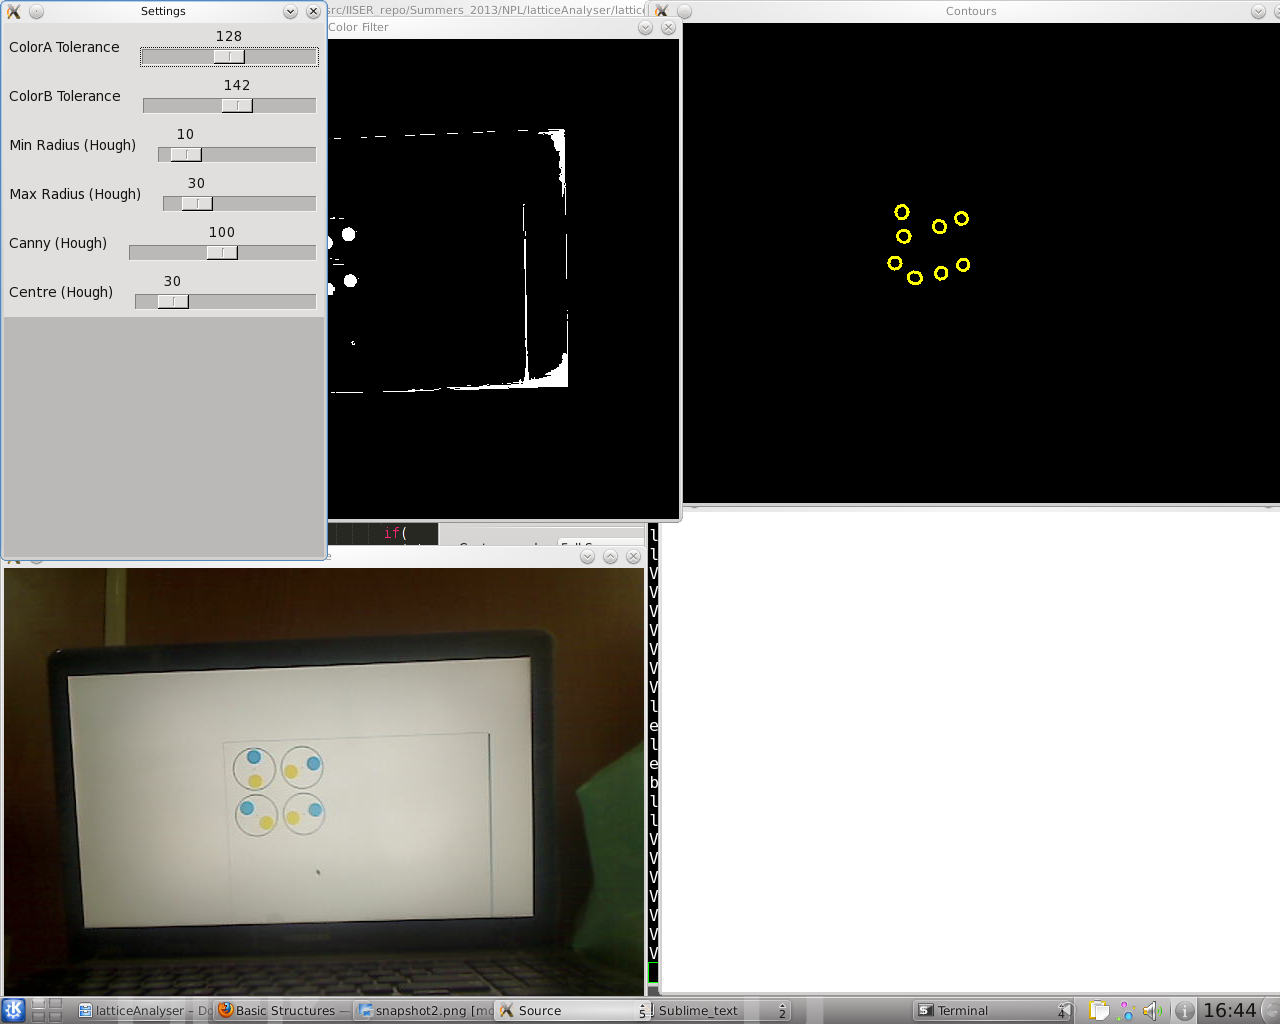
\includegraphics[width=1.1\linewidth]{../../latticeAnalyser/screenshots/snapshot2.png}
				\end{center}
			\caption[Contour Detection]{Contour Detection}
			\label{snapshot2}
			\end{figure}

			Next, a colour filter was to setup to improve the accuracy. When the algorithms were implemented, it was found that the Hough Transform method often misses detection of circles, refer to \autoref{snapshot1} (this is ofcourse after attaching a video stream instead of images to the code) as compared to contour detection \autoref{snapshot2}.
			\par

			\begin{figure}[bth]
				\begin{center}
					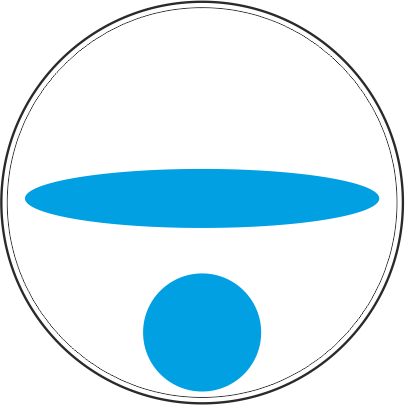
\includegraphics[width=0.3\linewidth]{../../latticeAnalyser/multimediaFiles/singleDipole.png}
				\end{center}
			\caption[Final Pattern]{Final Pattern}
			\label{singleDipole}
			\end{figure}

			\begin{figure}[bth]
				\begin{center}
					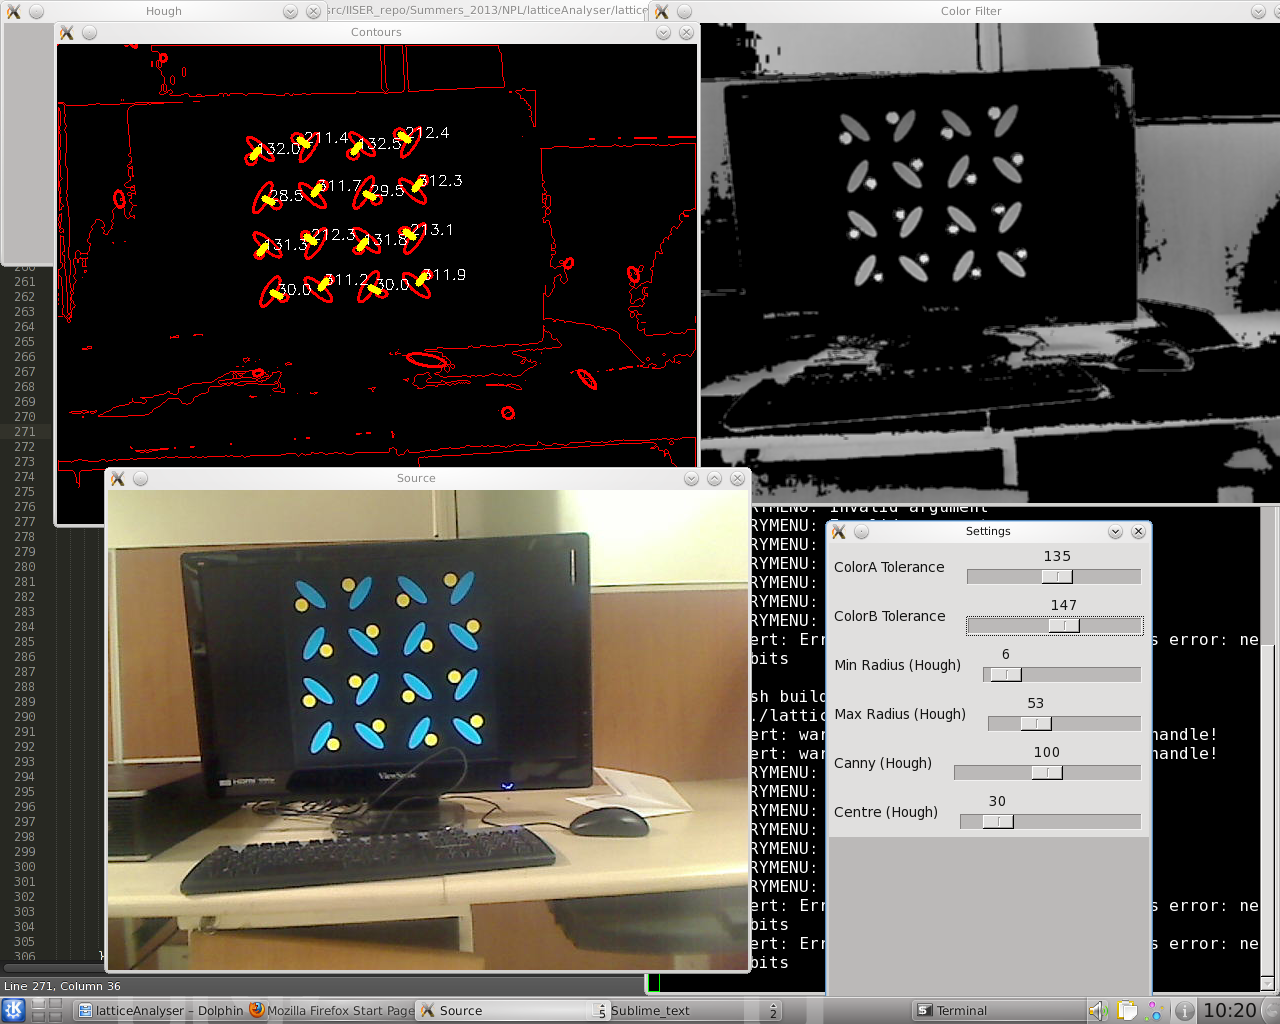
\includegraphics[width=1.1\linewidth]{../../latticeAnalyser/screenshots/snapshot5.png}
				\end{center}
			\caption[Multi Shape, Single Colour]{Multi Shape, Single Colour}
			\label{snapshot5}
			\end{figure}

			After the detection, according the plan, two colours were to be used for the ellipses. However, running the hough transform twice would've dropped the detection speed to half, which wasn't worth it. It was then decided that the shapes should be made different instead of relying on two colours for the same information. After looking at various combinations, \autoref{singleDipole} was finalized, with an ellipse at the centre, and a circle along the minor axis for breaking the symmetry. This method did infact work as shown in \autoref{snapshot5}.
			\par

			\begin{figure}[bth]
				\begin{center}
					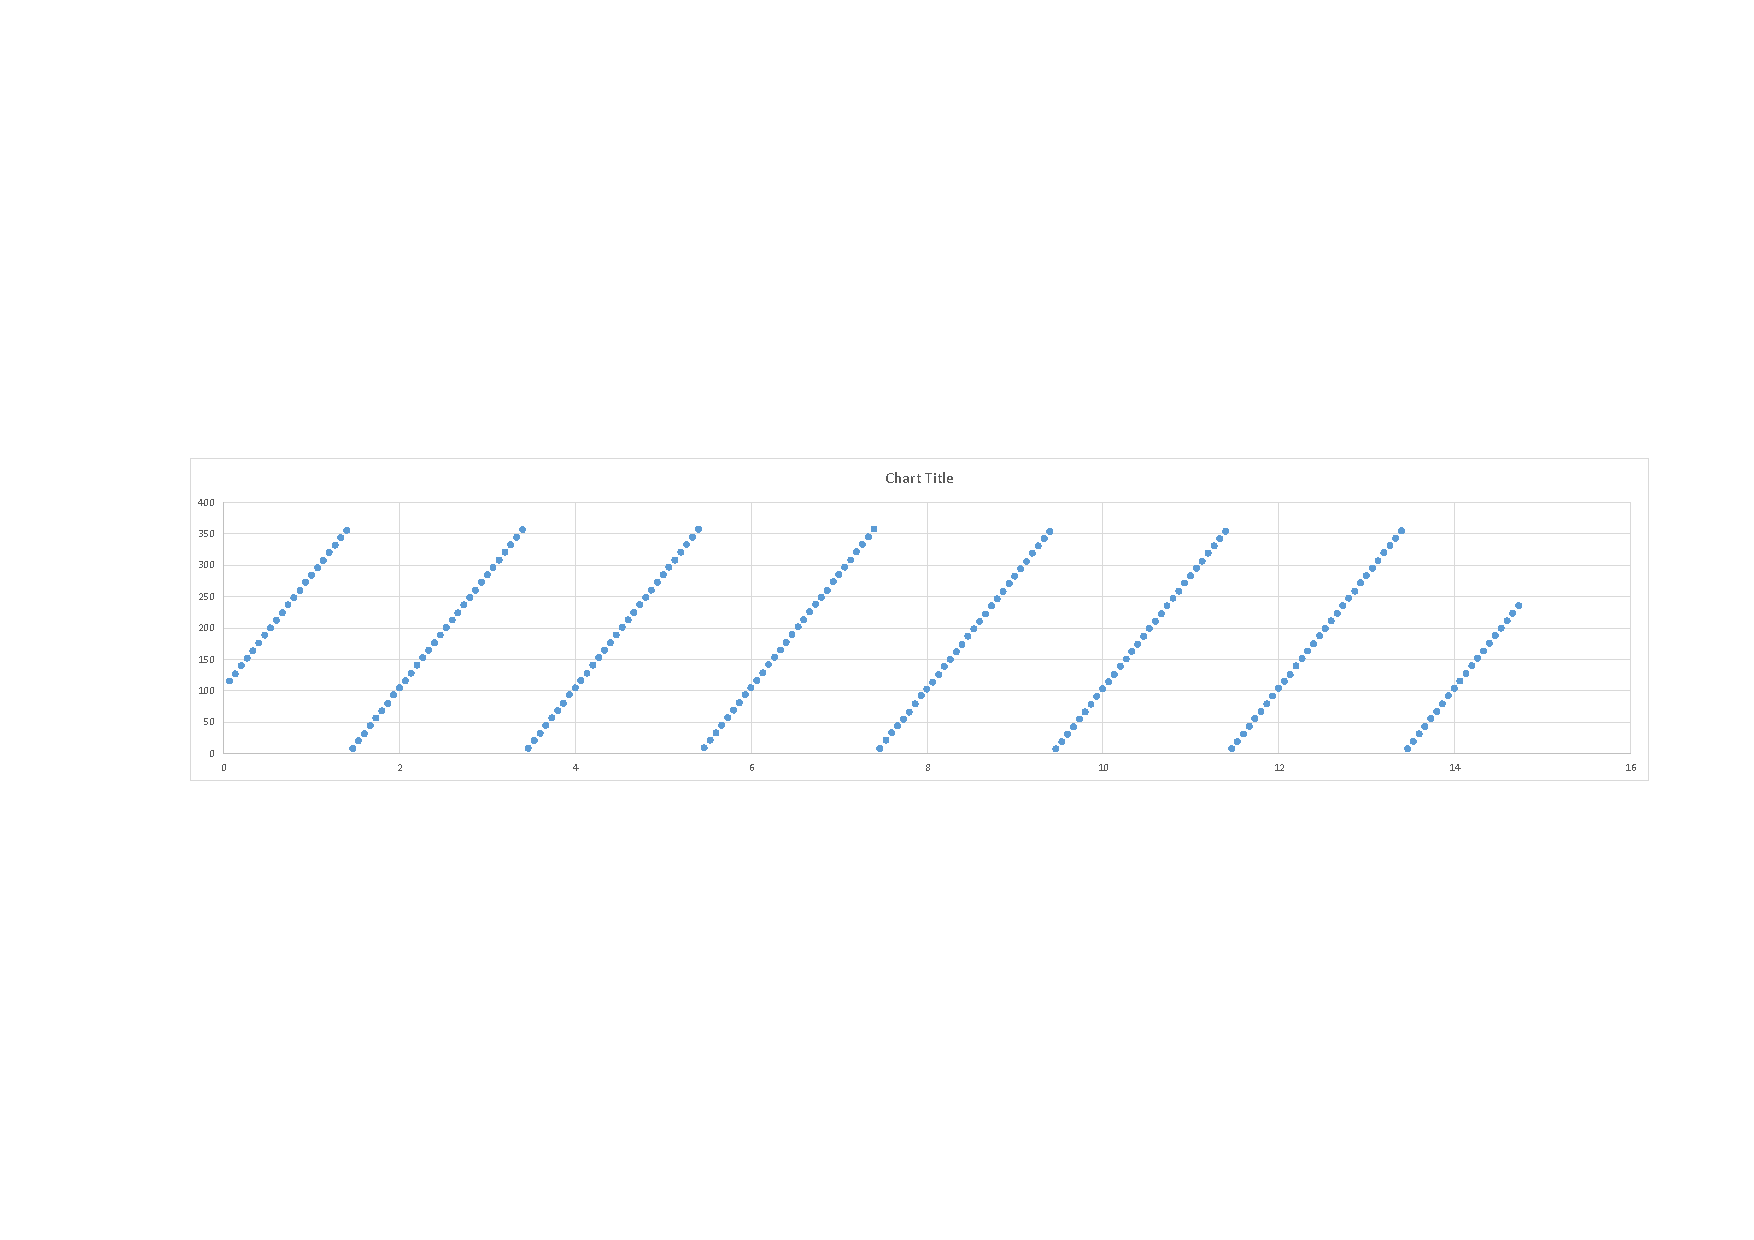
\includegraphics[width=1.1\linewidth]{gfx/testGraphs}
				\end{center}
			\caption[First Observation]{First Observation}
			\label{testGraphs}
			\end{figure}
		\subsubsection{Aftermath and Recognition Tests}
			The next challenge was to realize that a dipole detection can be missed and therefore mess up the counting, if that is the only way of uniquely identifying them. Unique identification is obviously required, as the external hardware must fire the coils of the right dipole. Thus a reference frame was used to uniquely identify the dipoles initially. This is expected to happen when they are stationary to get a good reading. In each frame, whenever a dipole is detected, it is associated with the dipole in the reference frame, by matching its location. If a dipole is not detected in a given frame, the software knows it was unable to record it and doesn't mess up neither the numbering nor the observations.
			\par

			\begin{figure}[bth]
				\begin{center}
					
\includegraphics[width=0.7\linewidth]{gfx/ellipseCircleDipoles4x4_black.jpg}
				\end{center}
			\caption[Final Test Pattern]{Final Test Pattern}
			\label{testPattern}
			\end{figure}

			After implementation of the last part, an animation sequence was created in Power Point, with the dipoles rotating with a constant speed and the camera was aimed at the screen. A still from the same is given in \autoref{testPattern}. \autoref{testGraphs}, shows the angular position versus time plot, for the first dipole and yes, it is linear, just as expected. Standard deviation tests are still to be done.
			\par
			Further tests, relating to it's timing were done and it was found that the processing itself was taking longer than the time taken by one frame in a 30 FPS video stream. This could be improved with the following
			\begin{enumerate}
				\item Intel Performance Primitives (IPP)
					\par
					These are libraries that provide optimized algorithms for performing some of the basic tasks in OpenCV to speed up the overall computation
				\item Multi Threading
					\par
					Rendering the frames in a different thread could perhaps increase the render speed or atleast ensure it doesn't affect the rate of processing of the image
				\item Camera Initial Delay
					\par
					Despite a 30 FPS smooth video, there seemed to be an initial delay which persisted in the video preview of the camera. This can be corrected for by polling the camera quickly instead of processing the image each time.
				\item OpenTBB
					\par
					To enable multi-threading within OpenCV to speed up the algorithms
				\item Hardware
					\par
					The results obtained earlier were for a Pentium 4 HT system. A faster multi-core processor could produce potentially, better benchmarks.
			\end{enumerate}
			Painstakingly, IPP was downloaded, built and integrated with OpenCV and re-built. There were various issues, starting from an incompatible version of IPP, to faulty documentation in OpenCV. The results did not improve however despite this. Perhaps the algorithms used do not rely on the methods optimized by IPP
			\par
			Multi-threading was implemented using C++ 11. Various synchronization methods were looked up, including mutexes, uniqe locks; eventually atoms were used and tested with Visual Studio Express 2012 on windows (implicitly implying the application was first made to run on windows), as the linux machine had an older kernel and upgrading GCC wasn't recommended.
			\par
			The camera's initial delay is caused by the initial stream. To rectify this, OpenCV has two methods, one for grabbing a frame, and the other for decoding it. If in a separate loop, the camera is polled regularly for frames, the delay is minimized. The frame can be decoded as soon as processing of the previous frame is over. This, as is suggestive, also requires multi-threading
			\par
			OpenTBB is a library that is required to enable multi-threading support in OpenCV. This too had to be fiddled with for a while, before being built successfully.
			\par
			The hardware was changed to an i7 machine which has more then enough cores and computation power.
			\par
			These modifications were all combined and the code compiled using GCC (except certain parts of multi-threading, due to a compiler issue) and it was found to be able to process in about 25 milliseconds for an $8 \times 8$ matrix of dipoles. For a $16 \times 16$ matrix, the resolution of the camera (Logitech Pro 9000, $640 \times 480$ at 30 FPS) was found to be insufficient. Higher resolutions in the same camera did not have a 30 FPS temporal resolution. The alternative seems to be a camera for the Rasberry Pi which can be used over ethernet.
			\par
			Further, the CLI of the program was modified to add support for inputting various commands, which would be required for testing the hardware (which is scheduled to be built this week).
		\subsubsection{`temperature' compatible}
			\par
			And surprise surprise, the hardware interface was in fact done in the following week. \myProf had already created a simplified version of the Ob-Dev firmware for USB interface of an Atmega with the PC which was used. More on that is there in the temperature section (which follows). The Lattice Analyser had to pump in energy to the system by providing angular velocity to the system of dipoles repetitively at suitable time intervals, viz. when the temperature of the system drops. The temperature is calculated in realtime using the RMS angular velocity of each dipole in the system. It was immediately realized after a closer look that since the time window between two frames is roughly 30 ms, it is not possible to energize all the dipoles with velocities picked from a given distribution of temperature. Further, since the motion of the entire system is coupled, it suffices to energize \emph{some} dipoles sufficiently to maintain the temperature.
			\par
			To achieve this the following were done (or algorithms for achieving them written) \footnote{For completeness sake, it must be stated that some modifications had to be made before the colour filtration became functional}
			\begin{enumerate}
				\item The tools for compiling and programming the AVR installed
				\item Bootloader programmed into the micro-controller along with the sample program given by \myProf
				\item Communication with the PC was tested using the corresponding C example program for the PC
				\item USB libraries were incorporated into the latticeAnalyser and linked (had to compile C objects with C++ objects)
				\item A simple IO protocol between the Lattice Analyser and the microcontroller was written and tested.
				\item The coil of a dipole was tested with a set of 4 A4 batteries and some basic current calculations were done
				\item The hardware was setup to include a small current limiting resistor (about 120 ohms) and the coil powered using the Lattice Analyser
				\item (was not required) Worked on sachetIO; a library for breaking down a large chunk of data into sachets intended to be transmitted and combined after being received.
				\item (was not required) Looked up methods to amplify the current, since the micro-controller's current wasn't found to be strong enough to align the needle of the dipole to it.
				\item Discussion about how to implement the energy pumping (which is how the previous two steps were found to be pointless)
				\item A $2 \times 2$ lattice of dipoles was setup. 
				\item The angular velocities of each dipole calculated
				\item With each frame, the RMS angular velocity calculated
				\item An algorithm for position and velocity based energy pumping written
				\item Interface added to test the same by supporting inversion of force direction (so that it results in halting) and an option to make blind (viz. disable the algorithm and instead send pulses periodically in time)
			\end{enumerate}
			The final result was that energy could be pumped into one dipole satisfactorily. The next step was to extend the algorithm to an arbitrarily sized matrix. Certain steps such as velocity calculations when dipole detection fails (at high speeds) has arbitrary inaccurate behaviour in the said version. Algorithms for finding the axis of the coil in the dipoles also needs to be finalized, for there are more than one ways of doing this, viz. powering the coils and reading the angular position of the dipole, finding the axis of the lattice by noting the Cartesian positions of the dipole, deduce it from the rest (initial) angular position of the dipoles which should be known given the lattice size, etc.				
		\subsubsection{Adding Realtime Graphing Capability}
			Before working further on the aforesaid steps, realtime graphing was implemented. This was thought to be required for \emph{seeing} what was happening, specially the angle detection and when it goes wrong. This is being emphasized because the angle detection would often result in incorrect angle calculation which was a serious issue.
			\par
			After searching the internet for plotting methods, plplot was finalized as the graphing library to be used with C++. This was downloaded, built and installed. I wouldn't go into the implementation details, but would remark that it takes a little time to get everything up and running. The library supports various kinds of graphs. The two types of that were used for the project are
			\begin{enumerate}
				\item Realtime 3D plot
				\item Strip chart
			\end{enumerate}
			Further, the library provides multiple rendering options, of which for linux, a driver for the x11 graphics system was used for testing. In a single window all three graphs were created;
			\begin{enumerate}
				\item 3D: Angular Position vs Dipole ID vs Time
				\item 3D: Angular Velocity vs Dipole ID vs Time
				\item Stripchart: Average Square Angular Velocity (over dipoles) vs Time
			\end{enumerate}
			Of course, these graphs weren't all added at once; \autoref{snapshot8}, \autoref{snapshot9} and \autoref{snapshot11} tell the story. For the stripchart it must be remarked that it auto scales and shifts as the data flows in. This proved to be more useful than expected for debugging the mod problem (helped visually see the co-relation between other parameters and occurrence of the error). Further it was also useful in identifying periodic fluctuations (with a somewhat constant time period) in the third graph.
			\begin{figure}[bth]
				\begin{center}
					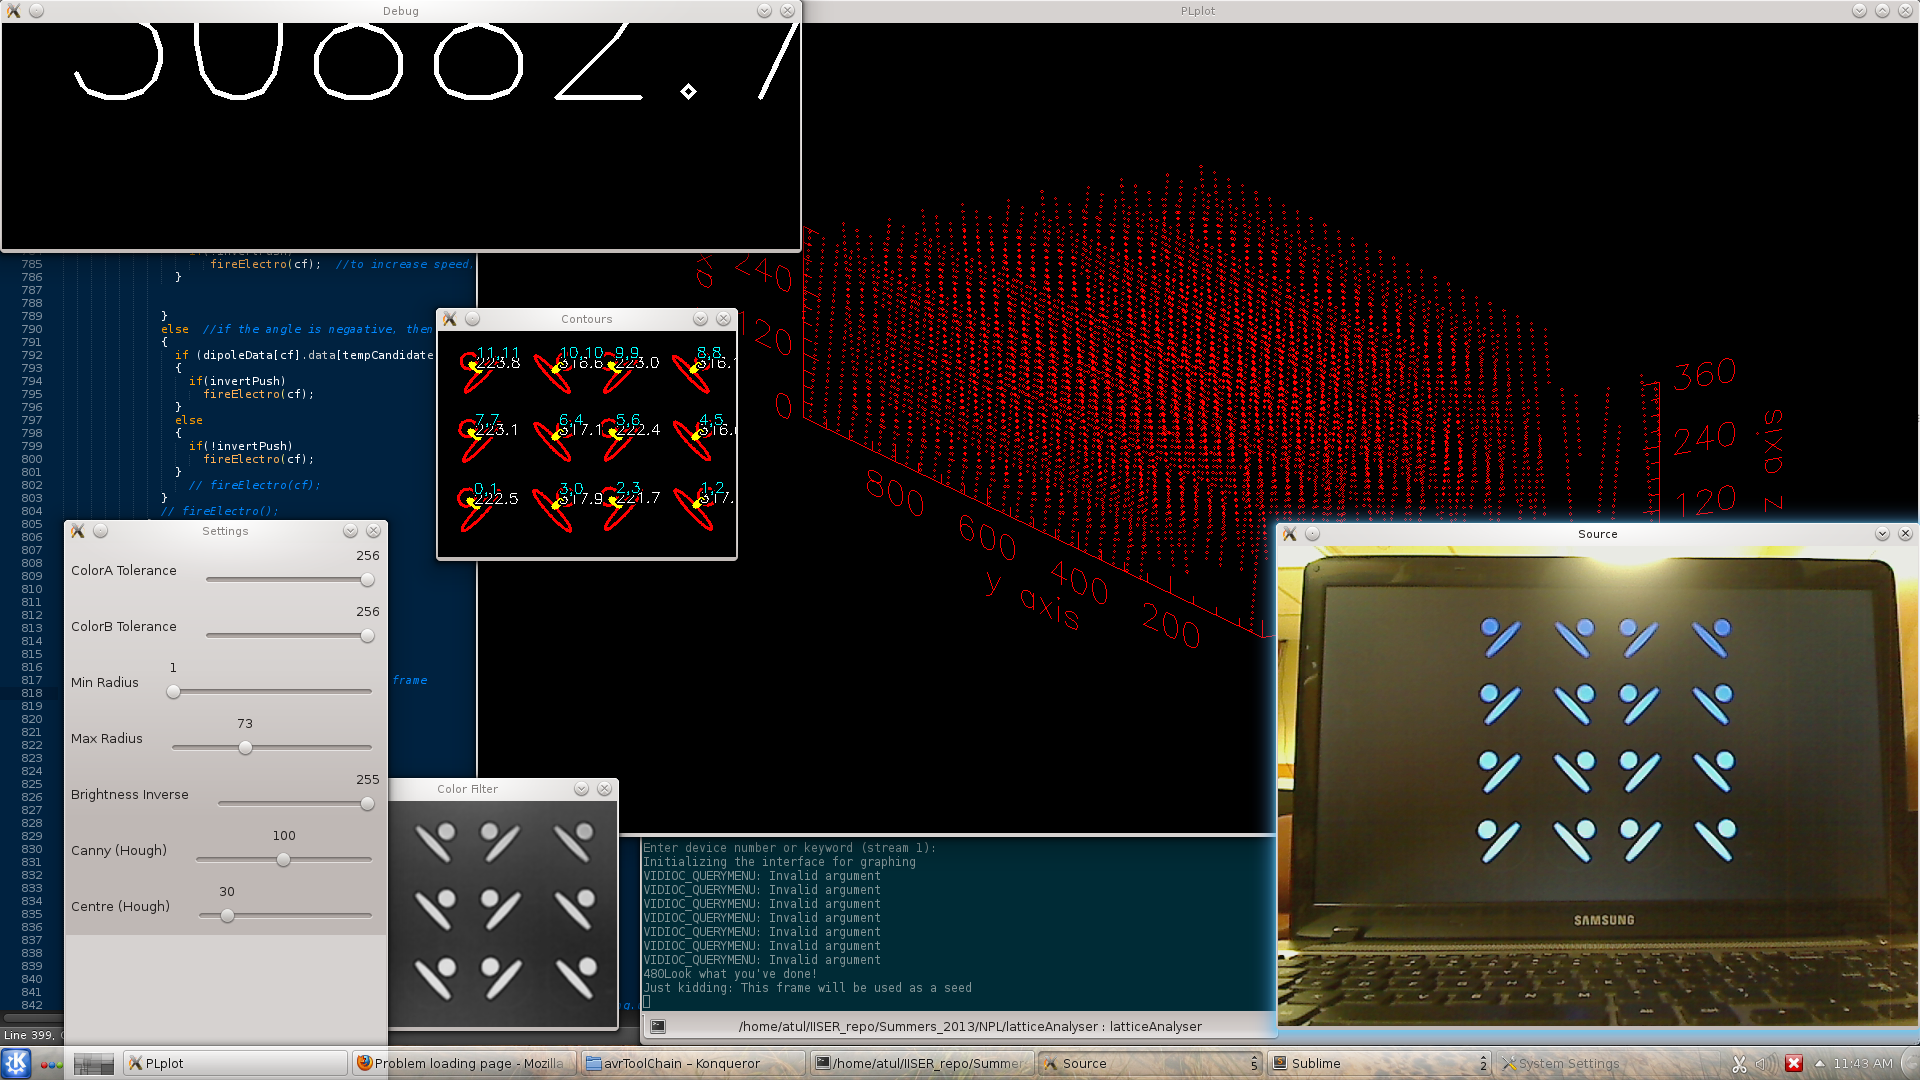
\includegraphics[width=1.1\linewidth]{../../latticeAnalyser/screenshots/snapshot8.png}
				\end{center}
			\caption[With the first graph]{With the first graph}
			\label{snapshot8}
			\end{figure}

			\begin{figure}[bth]
				\begin{center}
					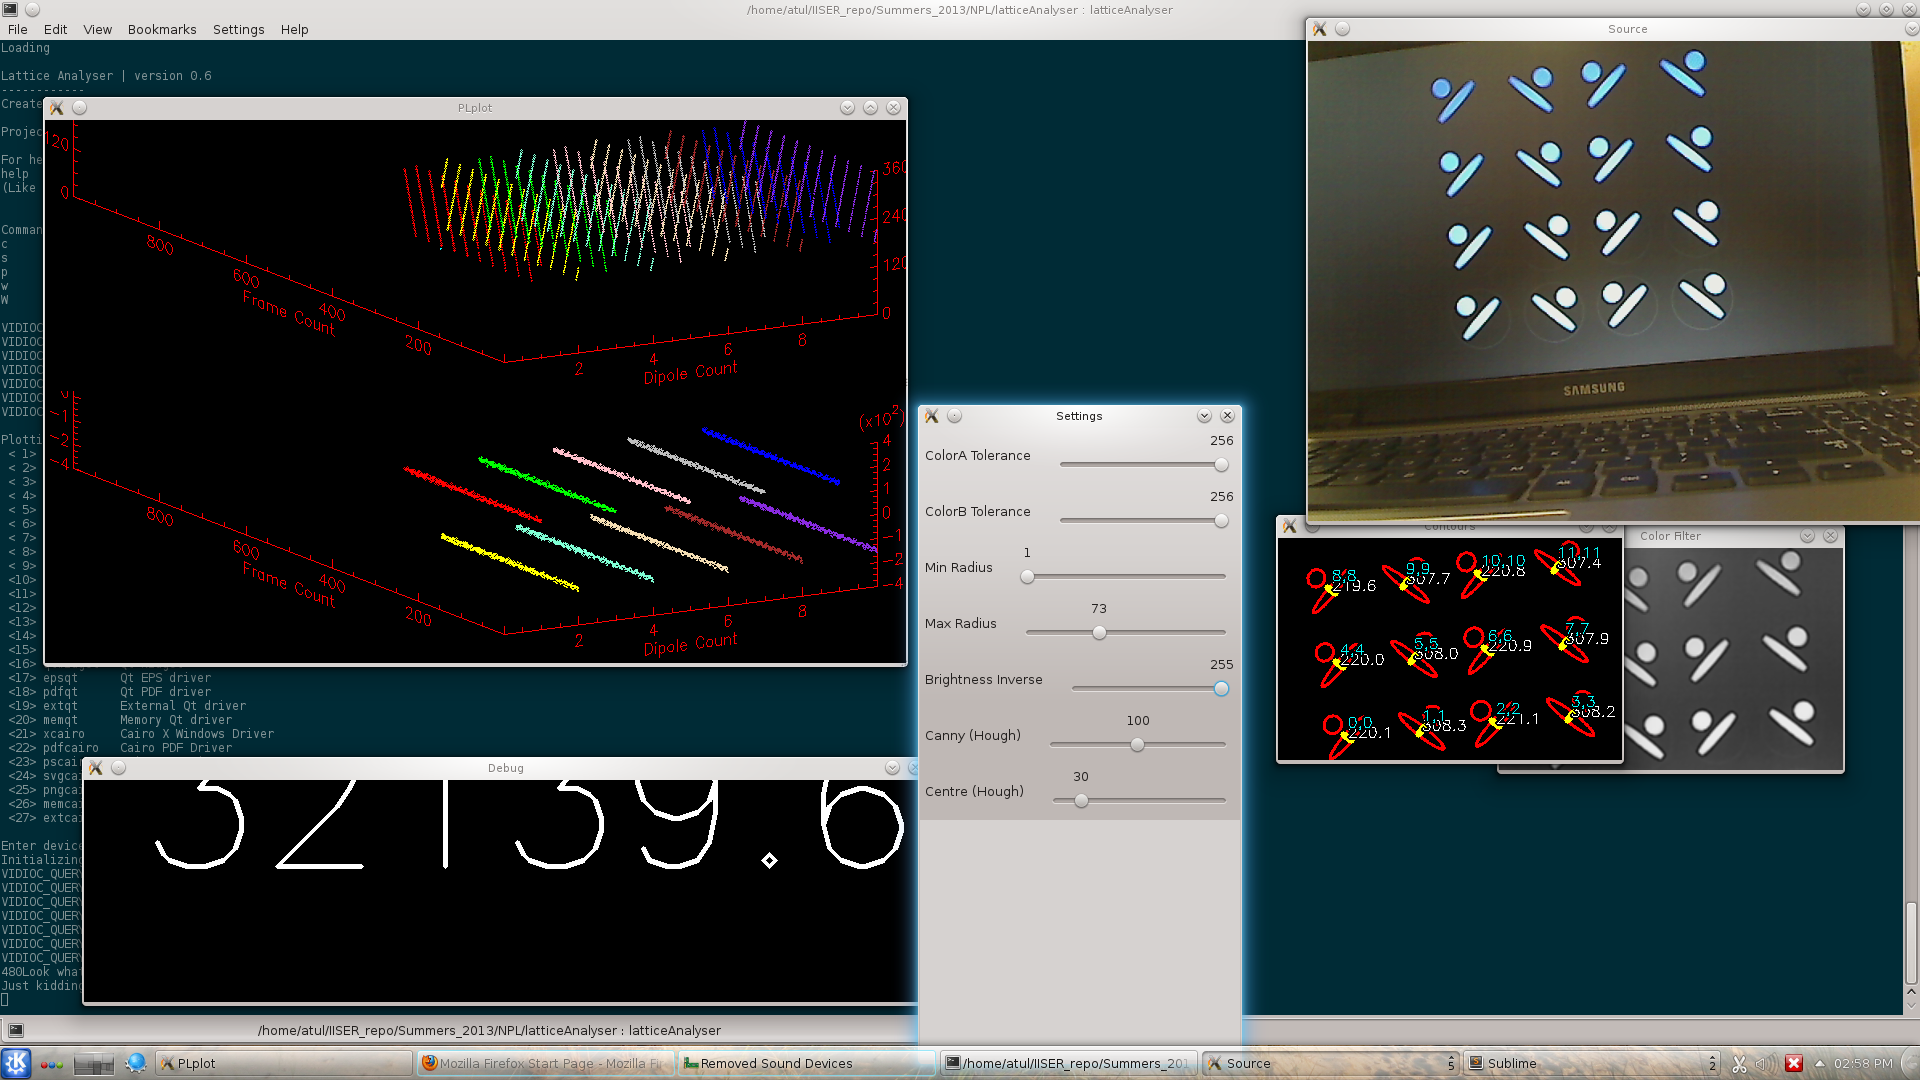
\includegraphics[width=1.1\linewidth]{../../latticeAnalyser/screenshots/snapshot9.png}
				\end{center}
			\caption[With the second graph]{With the second graph}
			\label{snapshot9}
			\end{figure}

			\begin{figure}[bth]
				\begin{center}
					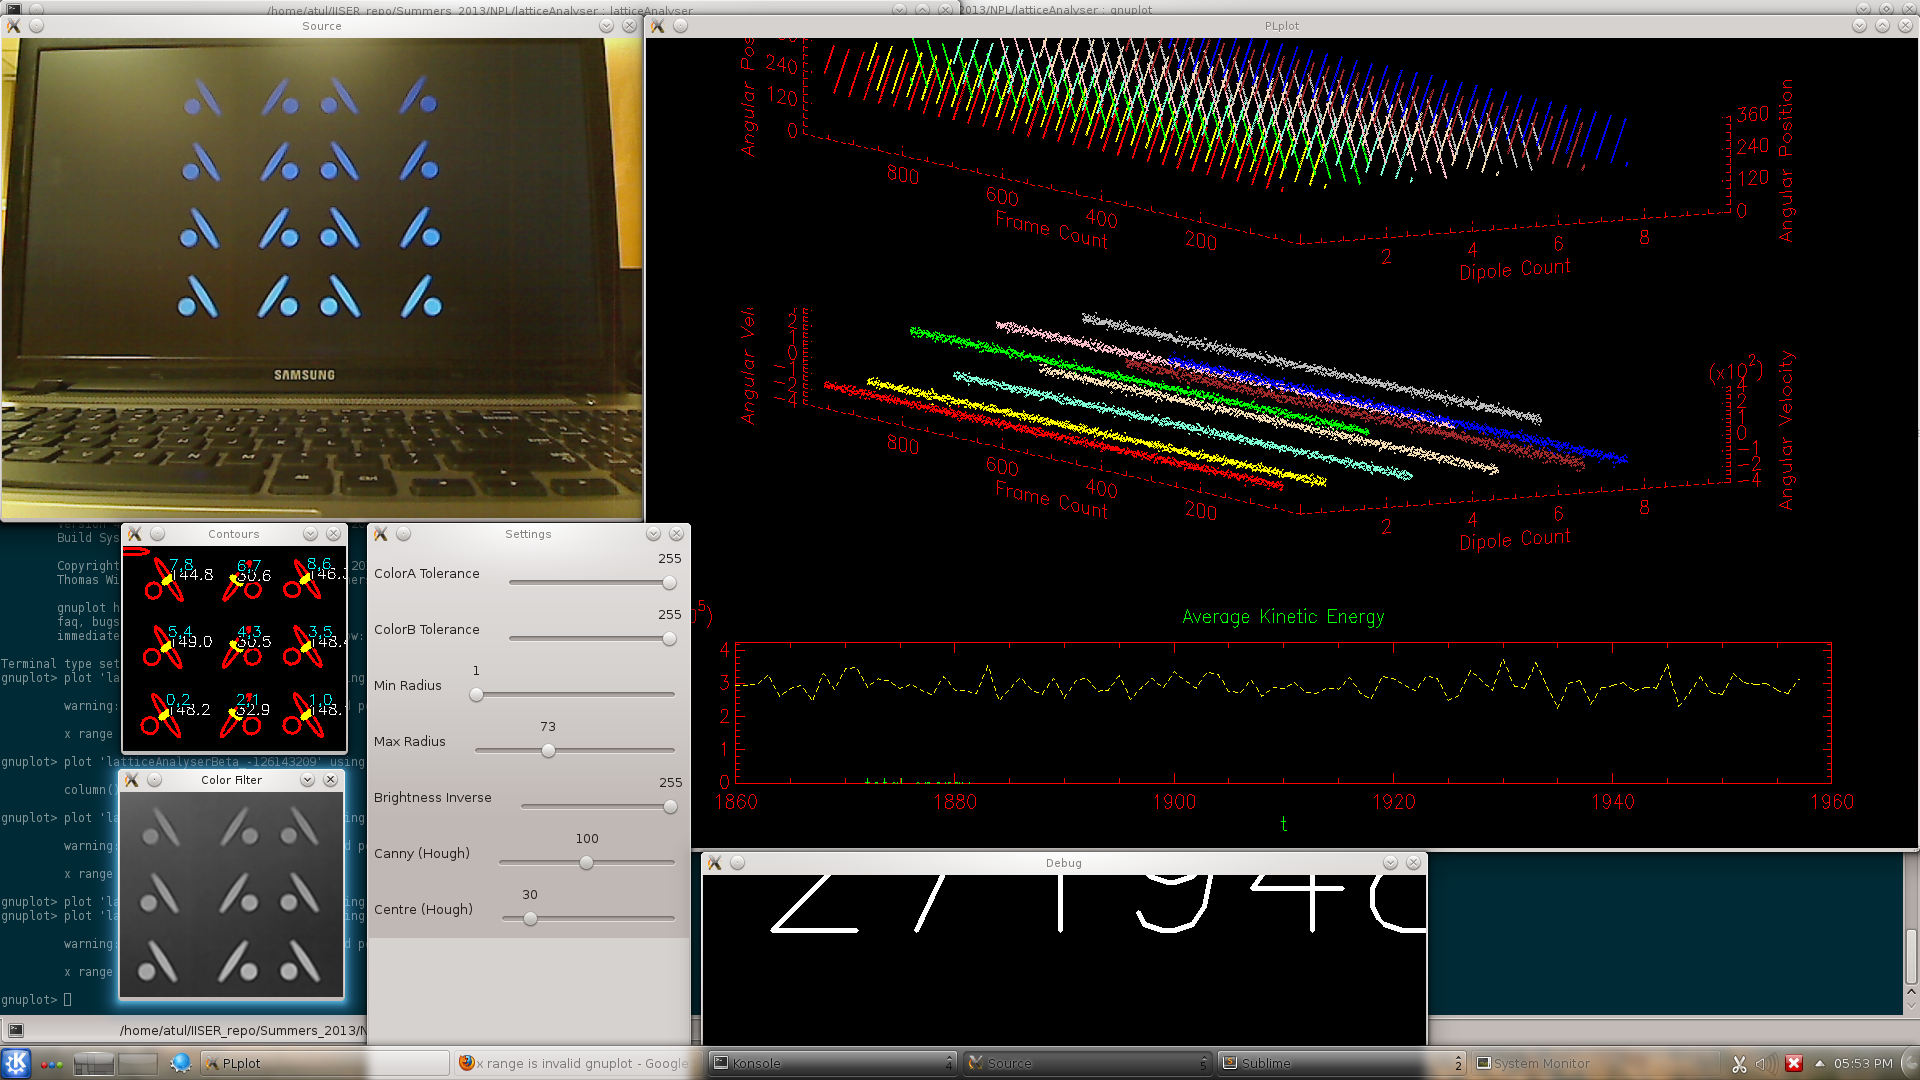
\includegraphics[width=1.1\linewidth]{../../latticeAnalyser/screenshots/snapshot11.png}
				\end{center}
			\caption[All the three graphs]{All the three graphs}
			\label{snapshot11}
			\end{figure}
			This will probably be the final user interface improvement for the Lattice Analyser.
		\subsubsection{The Modding Problem}
			Consider an ellipse. To describe all its orientations uniquely, given it's position, we need a convention for defining the angle and the angle should span pi radians. Only $\pi$ radians are required as opposed to $2\pi$ simply because of the symmetry of the ellipse. TODO: Put an image of an ellipse with the angle. We therefore need more information than the angle of the ellipse, to determine the angle of the dipole. The design of the pattern takes care of it by providing a circle to break the symmetry. Simplistically, the problem is now solved, for the circle's position can easily be used to decide when to add $\pi$ to the ellipse angle and you have the dipole's angle. TODO: Add an image showing the ellipse with a circle and the dipole angle changed accordingly.
			\par
			Upon implementing this simple logic as an algorithm and testing, it was found that it runs into troubles very quickly and periodically. To understand, first assume that the ellipse reads zero degrees when horizontal and thus, the circle, if it is above the 
			\par
			atan2 approximation for correcting the angle problem, atan2 assisted angle approximation, modular arithmetic based approach for correcting the dipole angle detection (figured this from a simpler problem of firing the elctromagnet)
		\\
		mod problem for deciding when to fire the electro magnet, used modular arithmetic
		\\
		RGB based colour detection to HSV based colour filtering, to improve high speed performance | various problems such as conversion of rgb to hsv and so on..
		\\
		misc: cmake was fiddled around with, auto numbering of lattice points, writing all the data into a file, gstreamer plugins for reading x264
		\\
		graph for kinetic energy added, there was a periodic shoot up, caused by modding problem
		\\
		testing source of systematic error, eliminating a cause, camera defect | calibration. list the two kinds of defects
		\par				
		PHYSICS:
		error analysis: used a lot of GNUplot, to test the kind of deviations for a given dipole, in the angle determination when static, when moving. Then for a given point of time, the deviation in the angles of various dipoles. damping could be tested with realtime grpahs

		The source code of the same is given in \autoref{latticeAnalyserMain}, which has been made available online.
		% \lstset{basicstyle=\footnotesize}
		% \lstinputlisting[language=C++,title=latticeAnalyser.cpp]{../../latticeAnalyser/latticeAnalyser.cpp}
	\subsection{temperature; the rise}
		`temperature' was built around the Atmega8 processor to start with. It's task was to energize the coils of the dipoles, when instructed by the Lattice Analyser. It's source code was written in C, compiled with the free AVR-GCC compiler using some other sister tools of it. Atmega's interface to the computer was built from \myProf's library, which was built to simplify the existing ob-dev's virtual USB libraries. The coils are powered directly using the chip for the $2\times 2$ setup. For larger matrices, a multiplexer will be required and built suitably.
		\par
		The current that was roughly enough to align the dipole to the coil was (after experiments with a 6 Volt battery and resistance of coil measurement, viz. 7 ohms) found to be about 1 ampere. The microcontroller can sync at most 20 mA of current at a given pin. Further for the USB interface, the system was set to run at 3.3 V (this can be pushed up to 5V also, but that would've required redesigning the circuit) and the current limiting resistor was correspondingly chosen to be about 150 ohms. This was put in series with the coil and tested. It was found that the dipole wouldn't, for even a second long pulse, align itself to the coil, starting from some initial angle. However, when further experiments were done for pumping in energy using the algorithms developed for the Lattice Analyser, this push was found to be enough, even with a few milliseconds long pulse. This version of temperature has been given in \autoref{temperatureFirstVersion}
		\par
		\begin{figure}[bth]
			\begin{center}
				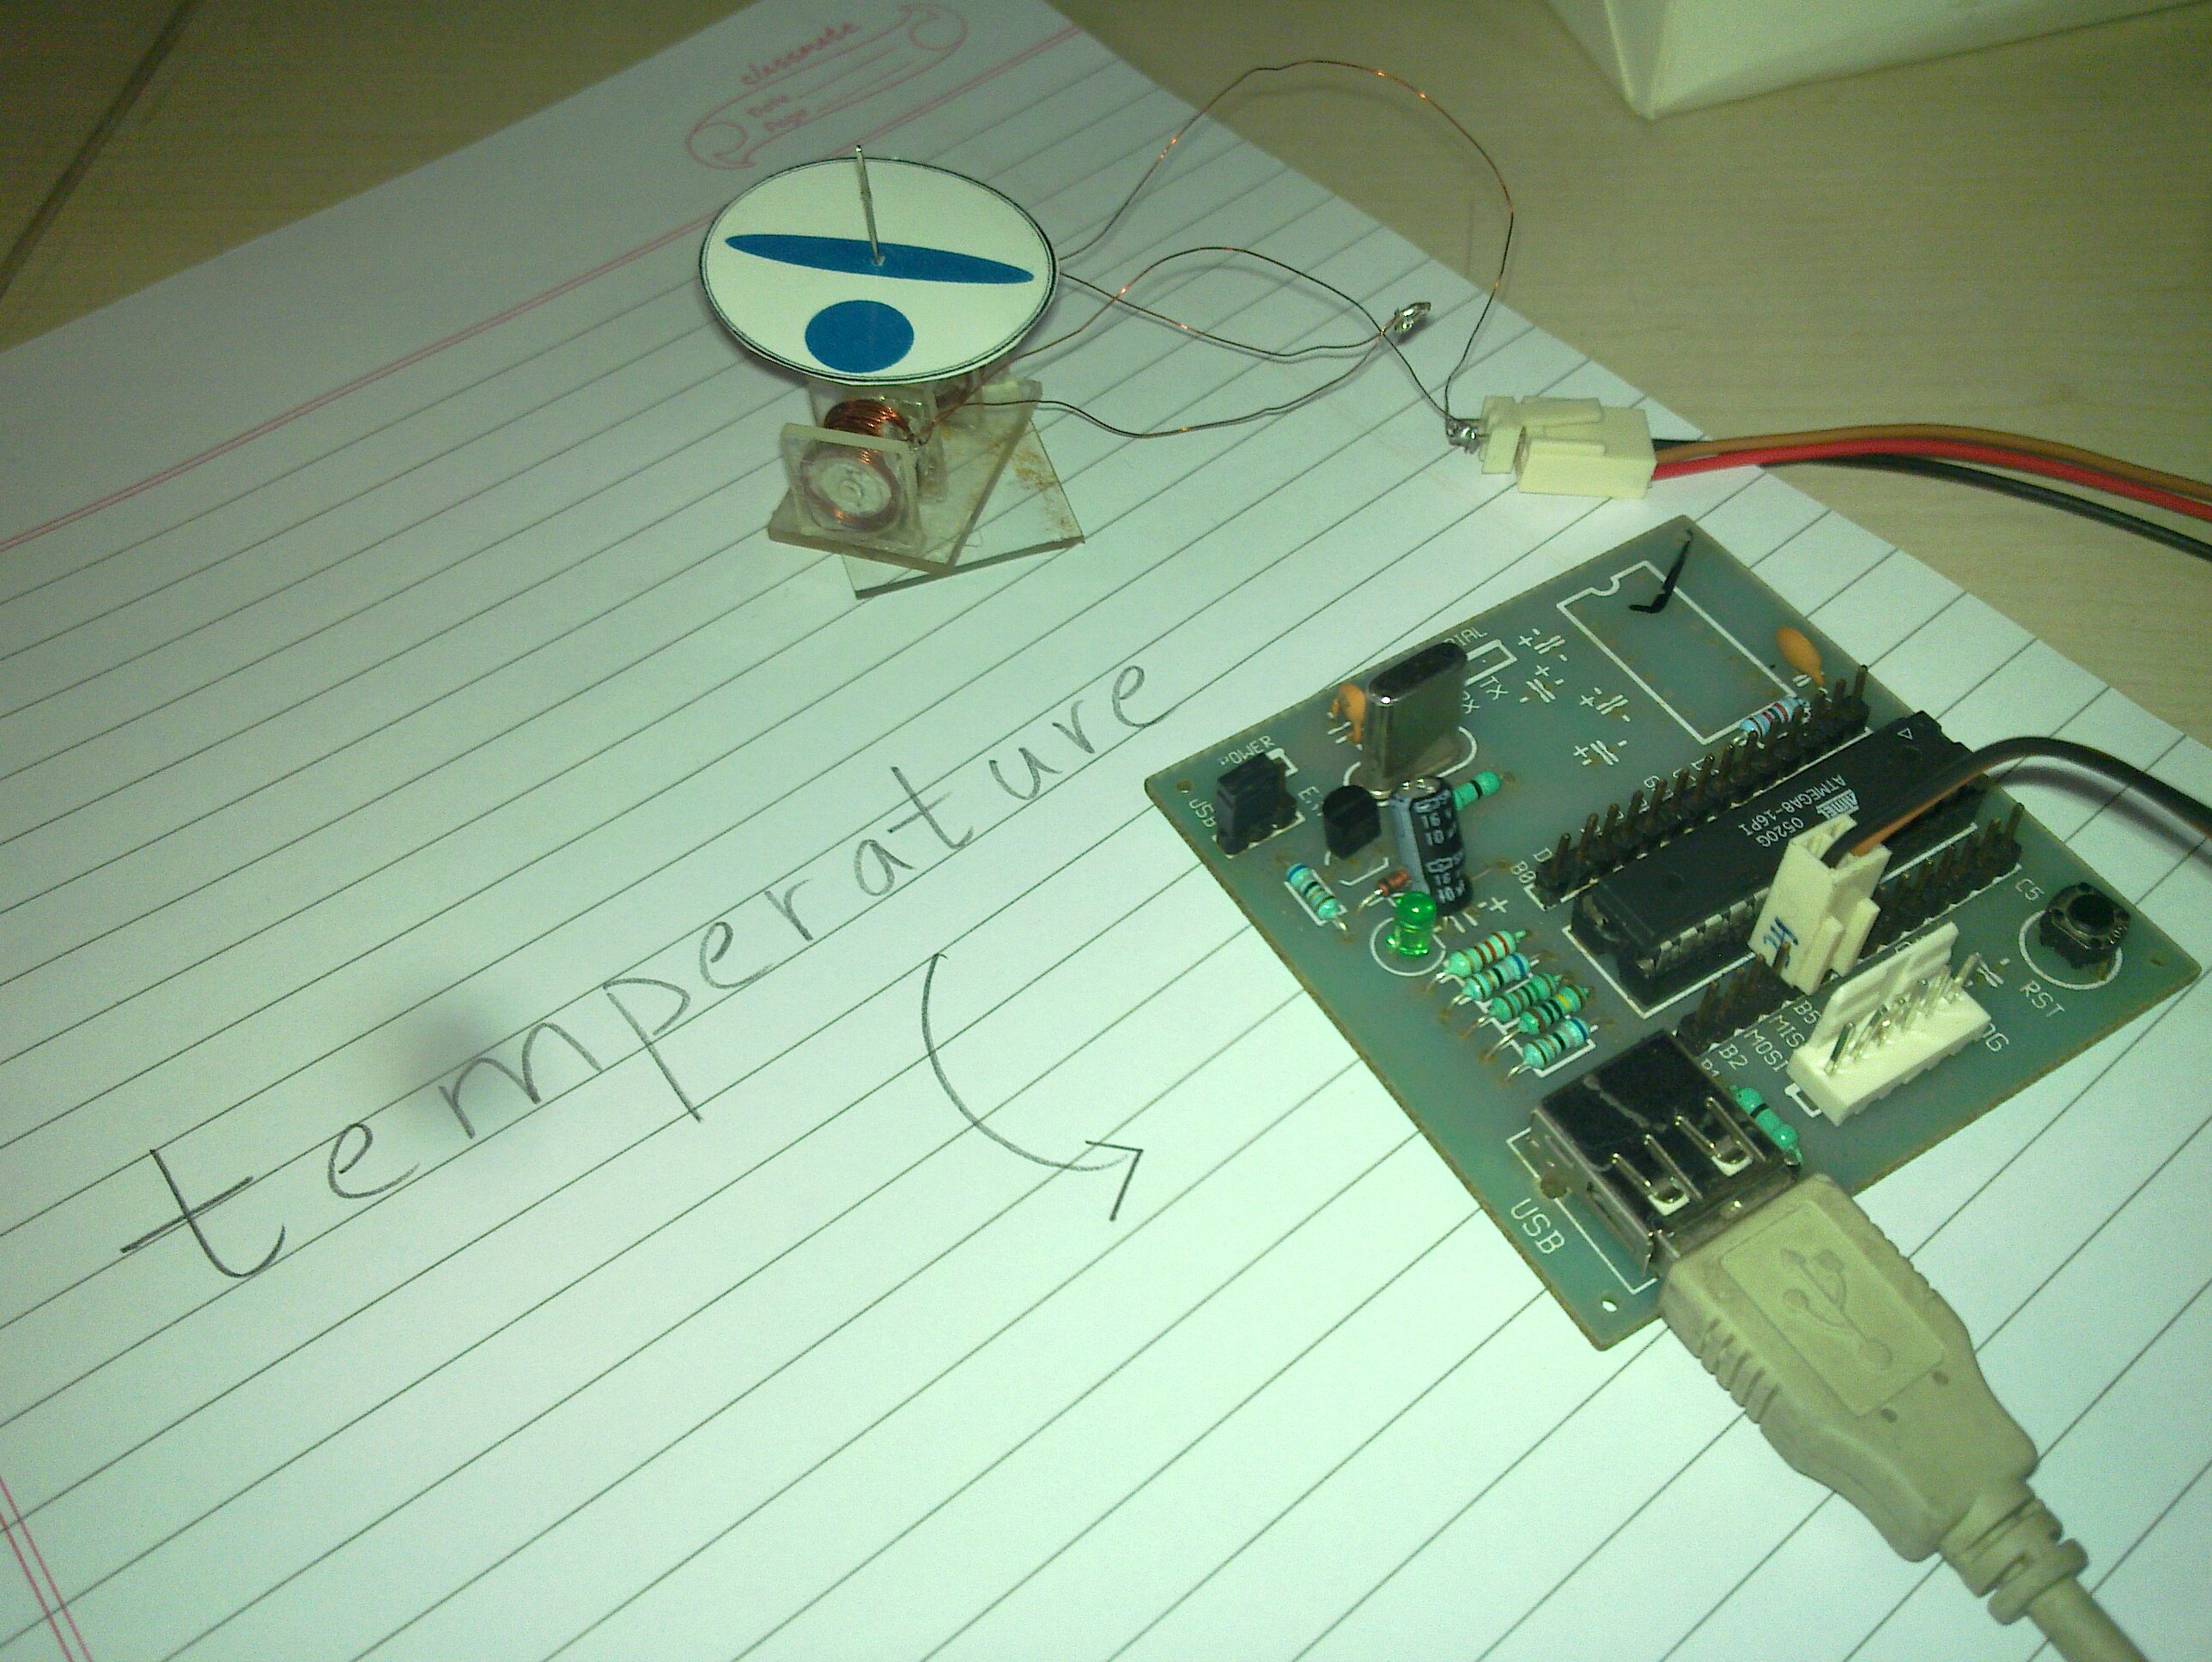
\includegraphics[width=0.85\linewidth]{gfx/temperature.jpg}
			\end{center}
		\caption[First Version of Temperature]{First Version of Temperature}
		\label{temperatureFirstVersion}
		\end{figure}
		\par
		The main file for the temperature has been listed in \autoref{temperatureMain}.
		% \lstinputlisting[language=C,title=tempereture.c]{../../temperature/firmware/temperature.c}
